\documentclass[fleqn]{tcdl}

\title{Introducción a la Materia}
\author[1]{Ernesto Bossi}
\affil[1]{Profesor}

\begin{document}

\flushbottom
\maketitle
\thispagestyle{empty}

\section*{Introducción}
\fontsize{11}{14}\selectfont

Los compiladores son programas informáticos que permiten traducir un programa escrito en un lenguaje, o en un archivo de entrada, en un programa escrito en otro lenguaje. Al mismo tiempo, un compilador es un sistema informático complejo, con varios componentes internos, algoritmos e interacciones entre estos componentes. Esta sección tratará sobre 
los componentes básicos que componen un compilador moderno.

\section*{Conceptos básicos de Construcción de lenguajes}

\subsection*{Nociones básica y motivación}

Los ámbitos en los que se ve una mayor uso de programas de computadora ha aumentado considerablemente en los últimos años, y no solo estos programas son utilizados por expertos o programadores, sino que en estos dias se ve un mayor uso de herramientas específicas,utilizadas por usuarios comunes. Además se ha visto el auge de hardware embebido que se ha utilizado para crear programas de uso específico en autos, aviones, teléfonos, etc. Estos programas son construidos a partir de otros programas que construyen herramientas virtuales, abstrayendo a los programas construidos de los detalles de bajo nivel de las computadoras que los ejecutan. Casi todos los programas son transformados a programas ejecutables por las computadoras llamados compiladores. En esta primera unidad mostraremos 

\subsection*{Estructura básica de un compilador}

Un compilador es una herramienta que nos permite traducir de un lenguaje de entrada a otro lenguaje de salida. Para traducir el texto de entrada de un lenguaje a otro, el compilador debe saber la forma, la sintaxis, el contenido o el significado (semántica) del lenguaje de entrada. También necesita conocer las reglas sintácticas y semánticas del lengaje de salida. Por último necesita un esquema, en el cual trabajar para el contenido de entrada de un lenguaje a otro.

La estructura gneral de un compilador generalmente deriva de esta descripción general e introductoria. Se dice que el compilador tiene un "front end", que se encarga de manjear el lenguaje de entrada. Y de un componente de "back end", que se encarga de generar el lenguaje de salida requerido. La conexión entre estos dos componentes, se hace formalmente por medio de representar el programa en una representación intermedia, cuyo significado es independiente de ambos lenguajes, pero en cuanto al significado, este mantiene el mismo que existía en el lenguaje de entrada. Para mejorar esta traducción, un compilador generalmente incluye un optimizador que analiza y reescribe esa representación intermedia.


\subsection*{Tipos de Compiladores}

Los programas informáticos son secuencias de operaciones abstractas escritas en un lenguaje de programación, un lenguaje formal diseñado para expresar operaciones computacionales. Los lenguajes de programación tienen propiedades y significados rígidos, en los cuales no se admite la ambiguedad. Un programa ambiguo no tiene significado. Las instrucciones computacionales son parte de una serie de tareas que producen resultados. 

Los lenguajes informáticos permiten a los programadores y usuarios el de expresar las tareas que desean realizar en una serie de operaciones, descriptas mediante una sintaxis propia del lenguaje que utilicen, y que es sencillo para el usuario de entender. Los procesos que ejecutan los microprocesadores, microcontroladores y cualquier tipo de máquina computacional física, están diseñadas para ejecutar una serie de operaciones. Estas operaciones están descriptas a un nivel de abstracción mucho más bajo que aquellos especificados para los usuarios. Por ejemplo, un lenguaje de programación puede tener en su sintaxis una manera muy concisa y simple de declararlo, sin embargo esta simple operación se puede traducir en cientos de operaciones al nivel de instrucciones de máquina que entienden las computadoras. La herramienta que hace esta traducción de un lenguaje de programación de alto nivel, a instrucciones de máquina, se llaman compiladores. 

Como se menciono en la sección anterior, un compilador se lo puede ver como una caja negra que toma un lenguaje fuente, y lo traduce a otro lenguaje:


\begin{figure}[h]
\captionsetup{type=figure}
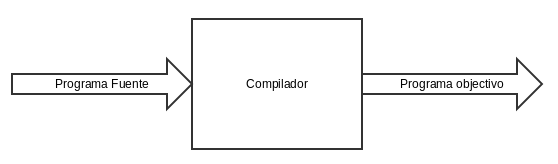
\includegraphics[width=\textwidth]{compilador_basico.png}
\caption{\label{fig:comp_basic}Caja negra de un compilador.}
\end{figure}


El lenguaje de entrada, es en general un programa en forma de texto de un lenguaje de alto nivel, como Java, C, ML, Ruby, etc y el lenguaje de salida es generalmente un conjunto de instrucciones de máquina.

Algunos compiladores traducen a un lenguaje objetivo que es en realidad un lenguaje que pueden leer los programadores o usuarios, en vez de un lenguaje de bajo nivel que entienden las computadoras. Estos programas, sin embargo, necesitan otra compilación si se desea que puedan ser ejecutadas. A este tipo de compiladores, se los llama traductores, y generalmente se usan en lenguajes de investigación o lenguajes descriptores de objetos para motores de juegos.


Otros sistemas diferentes al diagrama visto anteriormente califican como compiladores. Por ejemplo un lenguaje tipográfico que produce código PostScript puede ser considerado como un compilador. Porque toma una especificación de como debería verse un documento impreso, y produce un  archivo PostScript. PostScript es un lenguaje que describe imagenes. Debido a que el lenguaje tipográfico se traduce en un ejecutable PostScript, que pertenece a otro lenguaje, se dice que es un compilador. El código que transforma PostScript a pixeles, es tipicamente llamado un intérprete, no un compilador. Un Intérprete toma una entrada y produce como salida un resultado de la ejecución de ese programa de entrada.

\begin{figure}[h]
\captionsetup{type=figure}
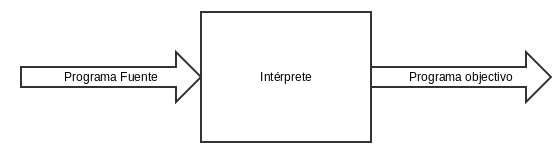
\includegraphics[width=\textwidth]{interprete_basico.png}
\caption{\label{fig:inter}Caja negra de un intérprete.}
\end{figure}

Algunos lenguaje adoptan un esquema de traducción mixto que incluye tanto compilación e interpretación. Por ejemplo, Java es un lenguaje que es compilado de su código fuente a una forma llamada bytecode, una representación compacta que esta pensada para disminuir los tiempos de ejecución en las aplicaciones construidas. Este bytecode que se genera en la fase de compilación es ejecutado en su correspondiente Java Virtual Machine (JVM), un intérprete de bytecode. La JVM, es en si una máquina virtual, que es una simulación de una máquina física con procesadores y memoria que permite abstraerse del hardware en el que se esta ejecutando este, e interpreta bytecode para generar resultados, por eso puede verse a la JVM como un intérprete. Muchas implementaciones de la JVM, implementan también un compilador que ejecuta en tiempo de ejecución del microprocesador físico, esto se los conoce como just-in-time-compiler o compiladores JIT.

Si bien los intérpretes y compiladores no son exactamente iguales, comparten mucho en común, ya que el módulo de "front end", es similar, tienen una manera de interpretar el lenguaje de entrada, obtener su significado y verificar previamente que este sintácticamente correcto, e incluso generan abstracciones que ayudan a conocer en que estructuras se guardarán valores intermedios del programa. Sin embargo la interpretación o "back end" final, difiere ya que un compilador genera una salida que es otro lenguaje o serie de instrucciones ejecutables que una vez ejecutadas producen una salida, mientras que los intérpretes en vez solo generan una salida directamente. En este curso se apuntará directamente a tratar sobre compiladores y bytecode, aunque también se mencionará sobre los distintos tipos de interpretación ya que son en si construcciones un poco más simples que las dos anteriores.

\subsection*{Principios fundamentales de la compilación}

Los compiladores son programas complejos y que deben ser diseñados e implementados cuidadosamente, un compilador que falla una vez cada tanto puede ser un proyecto inmaduro, pero inaceptable para ser usado en entornos productivos. Si bien muchos problemas pueden surgir y ser resueltos de varias maneras, dos principios siempre se tienen que mantener y siempre deben cumplirse. El primer principio es:
\\\\
\textit{El compilador debe preservar el significado o la semantica del programa que esta siendo compilado.}
\\\\
La correctividad es un tema fundamental en la programacion y un compilador debe mantener la correctividad del programa fuente de entrada. Este es el contrato principal que se tiene que cumplir entre el compilador y el usuario del mismo. 
El segundo principio es mas práctico y menciona que:
\\\\
\textit{El compilador debe mejorar el programa de entrada en una manera discernible.}
\\\\
Con esto se refiere a que el compilador, además de compilar el programa en si, debe proveer una manera de mejorar el programa de salida en cuanto a que debe ser lo más expresivo y si es posible, optimizar el programa de salida.

\newpage
\section*{Detalles de un compilador}
\fontsize{11}{14}\selectfont

Como se menciono en la sección anterior, el compilador tiene dos componentes principales uno en el que se maneja el lenguaje de entrada, "Front End", y que generará una representación intermedia, que permitirá después, al segundo módulo, "back end", generar el programa de salida, sea ejecutable, bytecode u otro programa codificado en un lenguaje de alto nivel. A continuación se muestra un diagrama de cajas negras:

\begin{figure}[h]
\captionsetup{type=figure}
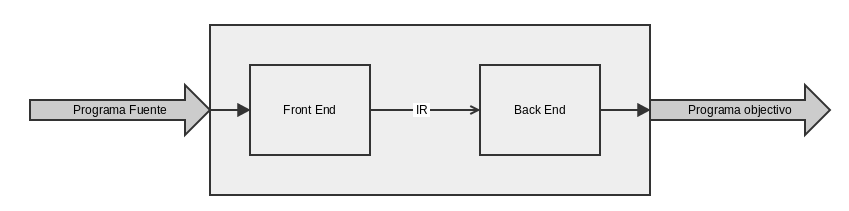
\includegraphics[width=\textwidth]{compilador_detallado.png}
\caption{\label{fig:inter}Caja negra de los componentes básicos de un compilador.}
\end{figure}

A continuación se muestra la figura de las fases que tendra la compilación, separando las fases de Front y Back End, con el detalle de cada subetapa:

\begin{figure}[h]
\captionsetup{type=figure}
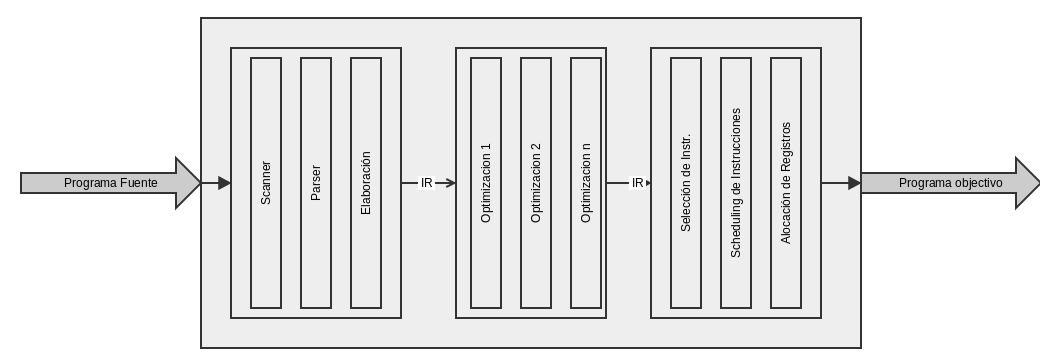
\includegraphics[width=\textwidth]{mucho_mas_detallado.png}
\caption{\label{fig:inter}Etapas de la compilación.}
\end{figure}
\bigskip

\subsubsection*{Etapas de la compilación}

\subsubsection*{Scanner}

Con respecto a la fase de Front End, se había mencionado que es la etapa en la que se detectará y validará tanto la sintaxis como la semántica del lenguaje de entrada, el objetivo es entonces el de generar una representación intermedia, como salida de este módulo, que luego se irá modificando en las optimizaciones que disponga el compilador, y será interpretado por el módulo de back end a fin de generar el programa de salida requerido por el usuario.
\\\\
En esta primera fase de scanning, se pasará la entrada por un Scanner, o tokenizador, que irá leyendo la entrada e irá separando la misma en pequeños objetos que luego utilizará el próximo proceso para determinar si la sintaxis es correcta, el scanner no validará que la sintaxis es la correcta, sino que solamente creará estos objetos que tendrán el valor de la entrada en partes indivisibles, a estos objetos los llamamos tokens o lexemas.


\subsubsection*{Parser}

El parser tomará la lista de tokens generados en el scanner, y los procesará a fin de determinar si la sintaxis de la entrada es la correcta o no. En caso de que no lo sea comunicará al usuario de este error y sino construirá una abstracción que representa en cierta manera el significado del programa de entrada. En general esta abstracción se encuentra representada en forma de árbol y esta será procesada por el siguiente módulo llamado, de elaboración. En general se utilizan los árboles de sintaxis abstracta para representar esta abstracción resultante del parser.


\subsubsection*{Elaboración}

El módulo de elaboración recorre la abstracción generada por el parser, generalmente un árbol de sintaxis abstracto, y permite a partir de este determinar cuestiones relacionadas con los contexto en el cual se definen variables, métodos, objetos y otras construcciones y se realizar el análisis semántico en el que se determina si el programa en cuestión tiene sentido. Luego esta capa genera la representación intermedia final, que luego tomará e interpretará el back end.


\subsubsection*{Optimizaciones}

Esta sección se tratará mas adelante y en la fase de optimizaciones se realizarán las optimizaciones que posee el compilador en un módulo intermedio para generar un código más optimo, estas optimizaciones se realizan a nivel de la representación intermedia.

\subsubsection*{Selección de instrucciones y Alocación de registros}

Esta primera etapa del backend, que se encargará de generar el código ejecutable o en otro lenguaje, trata de tomar cada una de las instrucciones de la reresentación intermedia y de acuerdo al contexto en la que estan enmarcadas, seleccionar las operaciones en código de máquina. Además de realizar esta operación, se realiza la alocación de variables extra, ya que en general los registros que tiene la representación intermedia son muchos más que la que existen en código de máquina, por lo que la traducción debe contemplar la alocación de registros o de reutilizar los registros utilizados en tiempo de ejecución y dejar en segundo plano aquellos que no se usen.

\subsubsection*{scheduling de instrucciones}

Para producir código eficiente, el generador de código debe reordenar las operaciones que reflejan las restricciones de performance de cada máquina. Cada tipo de de operaciones tiene un distinto tiempo de ejecución en ciclos, las operaciones de acceso a memoria puede requerir cientos de ciclos, mientras que las operaciones algebraicas entre registros pueden solo tomar algunas decenas de ciclos.El impacto del costo de las distintas operaciones puede ser dramático a la hora de generar código de máquina eficiente. varios procesadores tienen la propiedad en el que pueden iniciar nuevas operaciones mientras se ejecuta una una operaciones latencia larga. Tan pronto como los resultados de operaciones de larga latencia no son referenciados hasta finalizada su ejecución, la ejecución continúa. Por otro lado si alguna instrucción a futuro requiere de esta operación de larga latencia se demora su ejecución hasta que termine la primera instrucción. Una operación nunca empezará a ajecutar hasta que sus operandos estén listos y sus resultados no este listo hasta que la operación termina. El scheduler o administrador de instrucciones reordena las operaciones en el código e intenta minimizar los ciclos desperdiciados esperando nuevas instrucciones. Este reordenamiento debe producir el mismo resultado que el original.  

\end{document}